\section{形状坐标、测度与集体量子化}\label{sec:2-4}


第 1.2 节已经说明，强四极关联可以与 $I=0$ 态的球对称实验室一体密度并存。形变参考构型描述的是内部关联的一种组织方式，集体波函数则给出这些构型的量子叠加。这里进一步追问：选取形状和取向作为坐标以后，应怎样计算运动能量，又怎样解释波函数在形状空间中的分布？

本节先采用常正质量参数 $B$、五维欧氏四极坐标的教学 Bohr 模型。它使坐标、动能与积分测度之间的关系能够逐步推导；随后再说明一般惯性函数与量子化方案增加了哪些输入。五个坐标只保留四极自由度，并不完整表征核密度中的径向变化、高阶多极分量或质子—中子分布差异。


\subsection{从五个实坐标到形状与取向}\label{sec:2-4-1}


用无量纲球张量 $\alpha_{2\mu}$ 描述所选集体构型，其分量满足实条件

\begin{equation}\label{eq:2-4-1}
\alpha_{2\mu}^{*}=(-1)^\mu\alpha_{2,-\mu}.
\end{equation}

因此五个复球分量只含五个独立实自由度。为使欧氏范数显式成立，可选择

\begin{equation}\label{eq:2-4-2}
q_0=\alpha_{20},\qquad
q_{\mu c}=\sqrt{2}\operatorname{Re}\alpha_{2\mu},\qquad
q_{\mu s}=\sqrt{2}\operatorname{Im}\alpha_{2\mu},
\quad \mu=1,2.
\end{equation}

这五个实坐标满足 $\sum_a q_a^2=\sum_{\mu=-2}^{2}|\alpha_{2\mu}|^2$。其中 $\sqrt{2}$ 补偿了正、负磁分量在球张量范数中的成对贡献，速度范数也遵循同一关系。它们是集体构型的坐标，而非精确核态实验室密度的五个非零期望值。

例如，集体波函数可在许多取向的形变构型上都有振幅；恢复旋转对称性后，一体密度仍可为球对称。因此，从实验室态进入内禀坐标，并不是给核态指定一只已固定朝向的椭球。内禀坐标也可用来描述宽分布与振动，只有在分布足够局域时，单个参考构型才可能有效概括该态。

四极张量也可表示为实对称无迹矩阵。选其本征轴为内禀主轴，在这个坐标系中，球分量可取为

\begin{equation}\label{eq:2-4-3}
a_{\pm1}=0,\qquad
a_0=\beta\cos\gamma,\qquad
a_{+2}=a_{-2}=\frac{\beta\sin\gamma}{\sqrt{2}}.
\end{equation}

三个 Euler 角 $\Omega=(\phi,\theta,\psi)$ 描述主轴系相对于实验室系的取向；按本文的旋转约定，$\alpha_{2\mu}=\sum_\nu D^2_{\mu\nu}(\Omega)a_\nu$。由 $D^2$ 的幺正性，

\begin{equation}\label{eq:2-4-4}
\sum_{\mu=-2}^{2}|\alpha_{2\mu}|^2=a_0^2+2a_2^2=\beta^2.
\end{equation}

$\beta$ 因而是所选四极坐标的幅度，$\gamma$ 则给出内禀平面中的极角。这是坐标参数化，不是平移，也没有预先假定形状与取向的运动彼此独立。Bohr 原作以小幅核表面形变建立这一变换；它同样提示，具体密度与几何表面的对应仍有模型条件\cite{bohr-1952-surface-particle-coupling}。

主轴系并不唯一。一般三轴构型有六种轴序，每种轴序又有四种保持右手性的方向选择，共有 24 种等价重标记。它们组成旋转群 $O$，通过形状参数和 Euler 角的联合变换保持实验室四极张量不变。本文选择 $\beta\ge0$、$0\le\gamma\le\pi/3$ 作为形状扇区；六个形状扇区间的关系来自轴置换，不需要再借助空间反演。

对于固定轴序、三个本征值不同的构型，绕各主轴转动 $\pi$ 仍保持张量不变。这四种操作构成稳定子 $D_2$，所以限制形状扇区后，Euler 取向仍有这一冗余。若把空间反演也计入四极椭球的点对称操作，则得到八阶群 $D_{2h}$；它与 24 重主轴重标记具有不同含义。在轴对称端点，绕对称轴的连续旋转使稳定子进一步扩大；在 $\beta=0$，全部取向及 $\gamma$ 都失去唯一含义\cite{bohr-1952-surface-particle-coupling, prochniak-rohozinski-2009-bohr-collective-hamiltonian}。

下文固定轴号 $k=1,2,3$ 分别对应 $x',y',z'$。在小幅表面形变的轴长映射下，$\gamma=0$ 是以 $z'$ 为对称轴的长椭球端点，$\gamma=\pi/3$ 是以 $y'$ 为对称轴的扁椭球端点。$\gamma=\pi/6$ 是本文扇区的中点，三个轴通常不同；“中点”本身不定义适用于所有模型的最大三轴性量度。


\subsection{形状依赖的经典动能}\label{sec:2-4-2}


常 $B$ 模型从五个实欧氏坐标的动能出发：

\begin{equation}\label{eq:2-4-5}
T=\frac{B}{2}\sum_a\dot q_a^2
=\frac{B}{2}\sum_{\mu=-2}^{2}|\dot\alpha_{2\mu}|^2.
\end{equation}

对 $\alpha=D^2a$ 求时间导数，一部分来自 $a$ 的变化，另一部分来自主轴系旋转。主轴条件使这两类速度的内积为零。由于

\begin{equation}\label{eq:2-4-6}
\dot a_0^2+2\dot a_2^2=\dot\beta^2+\beta^2\dot\gamma^2,
\end{equation}

动能可写为

\begin{equation}\label{eq:2-4-7}
T=\frac{B}{2}\left(\dot\beta^2+\beta^2\dot\gamma^2\right)
+\frac12\sum_{k=1}^{3}\mathcal J_k(\beta,\gamma)\omega_k^2.
\end{equation}

这里 $\omega_k$ 是角速度在内禀主轴上的分量。没有形状速度与取向速度的交叉项，是这个二次型的性质；$\beta^2\dot\gamma^2$ 和形状依赖的 $\mathcal J_k$ 仍把各运动联系起来，不能据此把波函数普遍分解为互不耦合的因子\cite{bohr-1952-surface-particle-coupling}。

其物理意义可以从形状变化看出：即便某时刻只改变 $\beta$，转动惯量也随之变化，已有角动量对应的转动能因此改变。反过来，在给定角动量的通道中，不同构型的转动能会影响形状分布。把形状振动与转动写成两项，帮助辨认各类运动的来源，并不消除这种反馈。若要冻结形状，需再引入相应的近似。

转动几何因子可先从第三轴看出。绕 $z'$ 的微小转动使分量 $a_\nu$ 获得相位 $e^{-i\nu\,\delta\chi}$，因此相应速度范数的系数为 $\sum_\nu\nu^2|a_\nu|^2=8a_2^2$，得到 $\mathcal J_3=4B\beta^2\sin^2\gamma$。另两轴通过轴置换得到

\begin{equation}\label{eq:2-4-8}
\mathcal J_k=4B\beta^2\sin^2\left(\gamma-\frac{2\pi k}{3}\right),
\qquad k=1,2,3.
\end{equation}

这也是 Bohr 小幅、不可压缩无旋流模型中的惯量形式。它不是实核三条惯量的普遍经验定律。以 $\gamma=0$ 为例，$\mathcal J_3=0$、$\mathcal J_1=\mathcal J_2=3B\beta^2$；零分量反映绕对称轴改变取向不改变这个表面构型，不是说真实核不能拥有沿该轴的微观角动量\cite{bohr-1952-surface-particle-coupling}。

$\beta$、$\gamma$ 和 Euler 角均无量纲，故 $[B]=\text{能量}\times\text{时间}^2=\hbar^2/\text{能量}$，$\mathcal J_k$ 具有同一单位。用 $\hat j_k=\hat J_k/\hbar$ 表示无量纲角动量，可避免在转动能中遗漏 $\hbar^2$。这些惯量单位与电四极矩的电荷、长度平方单位无关。


\subsection{量子动能与积分测度}\label{sec:2-4-3}


常 $B$ 模型的量子动能在原实坐标中已经确定为 Cartesian Laplacian：

\begin{equation}\label{eq:2-4-9}
\hat T=-\frac{\hbar^2}{2B}\sum_a\frac{\partial^2}{\partial q_a^2}.
\end{equation}

设新坐标为 $y^i=(\beta,\gamma,\phi,\theta,\psi)$，将欧氏线元记为 $\sum_a\mathrm dq_a^2=h_{ij}\mathrm dy^i\mathrm dy^j$，其中 $h_{ij}$ 不含常数 $B$，$h^{ij}$ 为其逆矩阵。同一算符的坐标变换为

\begin{equation}\label{eq:2-4-10}
\hat T=-\frac{\hbar^2}{2B}
\frac{1}{\sqrt h}\sum_{i,j}
\frac{\partial}{\partial y^i}
\left(\sqrt h\,h^{ij}\frac{\partial}{\partial y^j}\right),
\qquad h=\det(h_{ij}).
\end{equation}

这是 Laplace–Beltrami 形式。度规系数随坐标变化，不会使原来平直的五维空间产生内禀曲率；此处的几何因素来自坐标网格。若另从一般坐标相关的经典质量张量出发，Podolsky–Pauli 构造是一种需要声明的量子化选择，不能仅由经典动能唯一指定全部量子修正\cite{prochniak-rohozinski-2009-bohr-collective-hamiltonian}。

从主轴本征值差得到的 Jacobian 含 $\beta^3|\sin3\gamma|$，内禀平面的极坐标变换再贡献一个 $\beta$；Euler 角则贡献旋转群的 Haar 因子 $\sin\theta$。吸收整体常数后，本节采用

\begin{equation}\label{eq:2-4-11}
\mathrm d\tau=\beta^4|\sin3\gamma|\,\mathrm d\beta\,\mathrm d\gamma\,\mathrm d\Omega,
\qquad
\mathrm d\Omega=\sin\theta\,\mathrm d\phi\,\mathrm d\theta\,\mathrm d\psi.
\end{equation}

若将 $B$ 纳入质量度规，其体积元还带常数 $B^{5/2}$；主轴重复覆盖及 Haar 元的整体归一也带常数。这些可一致吸收到波函数归一中，不改变概率，不能同坐标相关权重混淆\cite{prochniak-rohozinski-2009-bohr-collective-hamiltonian}。

在所选扇区内部，动能写为 $\hat T_{\mathrm{vib}}+\hat T_{\mathrm{rot}}$，其中

\begin{equation}\label{eq:2-4-12}
\hat T_{\mathrm{vib}}=-\frac{\hbar^2}{2B}
\left[
\frac{1}{\beta^4}\frac{\partial}{\partial\beta}
\left(\beta^4\frac{\partial}{\partial\beta}\right)
+
\frac{1}{\beta^2\sin3\gamma}\frac{\partial}{\partial\gamma}
\left(\sin3\gamma\frac{\partial}{\partial\gamma}\right)
\right],
\end{equation}

\begin{equation}\label{eq:2-4-13}
\hat T_{\mathrm{rot}}=\sum_{k=1}^{3}\frac{\hat J_k^2}{2\mathcal J_k}
=\frac{\hbar^2}{8B\beta^2}
\sum_{k=1}^{3}\frac{\hat j_k^2}
{\sin^2(\gamma-2\pi k/3)}.
\end{equation}

$\hbar^2/B$ 提供能量单位，其余导数和 $\beta$ 的幂次均无量纲。尤其 $1/\beta^2$ 是幅度依赖的几何因子，不能解释成物理长度平方的倒数。加上 $V(\beta,\gamma)$ 后，形状与取向仍通过同一哈密顿量决定量子态。

径向部分展开为 $\partial_\beta^2+(4/\beta)\partial_\beta$。第二项记录了随幅度增长的四维角向体积，不能在换坐标时省去。若只把笛卡尔动量换成 $-i\hbar\partial_\beta$ 后平方，就会得到另一种微分算符，并破坏它与所选内积的配合。体积元因而同时参与波函数归一和动能构造，不只是画概率图时的附加权重。

一般 Bohr 模型需要更多微观输入。Próchniak 与 Rohoziński 在综述中用三个振动惯性函数和三个转动惯性函数描述经典二次动能；它们通常依赖于形变坐标 $(\beta, \gamma)$。在由一般经典质量张量构造量子哈密顿量时，必须将平直欧氏空间坐标微分产生的几何因子 $\beta^4 |\sin 3\gamma|$，与依赖于动力学微观响应的质量张量行列式 $\sqrt{\det B(\beta, \gamma)}$ 严格区分开来。在 Podolsky–Pauli 构造下，内积权重与坐标依赖质量张量相耦合；而在更广泛的唯象或自洽集体模型中，动能二阶微分算符的逆质量系数张量与积分测度中的标量权重函数 $W(\beta, \gamma)$ 甚至可以独立指定，前一种关联仅为其特殊极限。在处理一般微观坐标依赖质量时，绝不能不加检验地直接沿用常 $B$ 模型下无额外质量权重的几何内积；具体一般形式与量子势修正留待附录 C 展开\cite{prochniak-rohozinski-2009-bohr-collective-hamiltonian}。


\subsection{坐标端点与波函数定义域}\label{sec:2-4-4}


采用上述归一约定，常 $B$ 模型的波函数满足

\begin{equation}\label{eq:2-4-14}
\int|\Psi(\beta,\gamma,\Omega)|^2
\beta^4|\sin3\gamma|\,\mathrm d\beta\,\mathrm d\gamma\,\mathrm d\Omega=1.
\end{equation}

在这个模型中，关于 $\gamma$ 的边缘概率密度还需积分掉 $\beta$ 和取向，并乘上 $|\sin3\gamma|$。单独画出 $|\Psi|^2$，尚不能把纵轴称为相对于 $\mathrm d\gamma$ 的概率密度。

取向与形状相关时，这一积分也包含不同转动分量的贡献，不能先假定波函数可分离再解释角分布。这里的概率是所选集体模型中的坐标概率；把它同电荷不变量、寿命或跃迁强度连接起来，还要指定相应算符，不能将模型边缘分布直接称为实验测得的连续核密度。

轴对称端点的 Jacobian 为零，表示部分取向坐标退化，不能据此添上一道物理硬壁。要使量子动能自伴，除微分表达式外，还要指定定义域，并使分部积分的边界形式在域内任意两个函数之间消失。有限概率流甚至某个态的零概率流，都不足以独自确定唯一自伴域。

对标量角向算符，该边界形式正比于 $\sin3\gamma\,[f^*g'-(f')^*g]$ 在两端的差，其中撇号表示对 $\gamma$ 求导。要求它对定义域中的任意 $f,g$ 都消失，比只考察一个波函数的流更强；还须使所选算符域与其伴随的域相配。这说明边界条件属于模型的量子定义，而非从测度归零直接读出的数值便利。

以 $I=0$、平坦角向势的标准正则分支为例，令 $x=\cos3\gamma$，则

\begin{equation}\label{eq:2-4-15}
\frac{1}{\sin3\gamma}\frac{\mathrm d}{\mathrm d\gamma}
\left(\sin3\gamma\frac{\mathrm d}{\mathrm d\gamma}\right)
=9\frac{\mathrm d}{\mathrm dx}
\left[(1-x^2)\frac{\mathrm d}{\mathrm dx}\right].
\end{equation}

相应正则本征函数是 $P_\ell(x)$，算符本征值为 $-9\ell(\ell+1)$。它们满足端点条件 $\sin3\gamma\,\mathrm d\psi/\mathrm d\gamma\to0$，同时 $P_\ell(\pm1)=(\pm1)^\ell$ 可以非零。这里选择的是由原坐标中正则波函数继承的分支，不是为所有集体问题证明了同一个边界条件\cite{bohr-1952-surface-particle-coupling}。

有转动分量时，还须满足主轴重标记的一致性，不能把所有分量一律置零。对于偶偶核的纯四极标量集体空间，$D_2$ 对称化可限制 Wigner 函数展开只含偶数 $K$；$K$ 在这里是所选主轴上的展开标签，三轴哈密顿量一般会混合这些分量，并不赋予全局好 $K$。在 $\beta=0$，不同角向通道也须共同恢复正则五维函数。加入奇核子或其它内禀自由度后，应重新构造包含它们的变换性质和定义域。


\subsection{平均形状角与动力学能标}\label{sec:2-4-5}


$V(\beta,\gamma)=V(\beta)$ 只说明势不依赖 $\gamma$，不表示哈密顿量在 $\gamma$ 平移下不变；动能中仍有 $\sin3\gamma$。在常 $B$ 模型的标准最低角向 $I=0$ 通道中，常数函数使非负角向动能达到零，因而成为这一通道的基态。

为单独观察角向分布，现限制在 $\beta=\beta_0>0$ 的角向模型上。这是受约束流形，不是将 $\delta(\beta-\beta_0)$ 当作完整五维可归一径向波函数。令 $M_\gamma=B\beta_0^2$，其平坦势动能为

\begin{equation}\label{eq:2-4-16}
\hat H_\gamma=-E_*\frac{1}{\sin3\gamma}\frac{\mathrm d}{\mathrm d\gamma}
\left(\sin3\gamma\frac{\mathrm d}{\mathrm d\gamma}\right),
\qquad E_*=\frac{\hbar^2}{2M_\gamma}.
\end{equation}

在 $\int_0^{\pi/3}|\psi|^2\sin3\gamma\,\mathrm d\gamma=1$ 的约定下，常数基态为 $\psi_0=\sqrt{3/2}$。变量变换需保留积分方向：

\begin{equation}\label{eq:2-4-17}
\mathrm dx=-3\sin3\gamma\,\mathrm d\gamma,\qquad
\int_0^{\pi/3}f(\cos3\gamma)\sin3\gamma\,\mathrm d\gamma
=\frac13\int_{-1}^{1}f(x)\,\mathrm dx.
\end{equation}

故 $p_x(x)=1/2$，而 $p_\gamma(\gamma)=(3/2)\sin3\gamma$。同一态在 $x$ 上均匀、在 $\gamma$ 上不均匀，并有 $\langle x\rangle=0$、$\langle x^2\rangle=1/3$；关于扇区中点的几何对称性直接给出 $\langle\gamma\rangle=\pi/6=30^\circ$。必须强调，该平均值完全源于几何测度因子 $\sin 3\gamma$ 在扇区中点取得极大的坐标网格效应，其概率峰并未借助任何动力学束缚势，绝不意味着体系处于具有三轴极小势阱的刚性转子极限。

也可把波函数改记为在 $\mathrm dx$ 下归一的 $u(x)=\psi(\gamma(x))/\sqrt3$。此时角向内积没有显式权重，但转回 $\gamma$ 后仍有 $p_\gamma=3\sin3\gamma\,|u(\cos3\gamma)|^2$。改变波函数的归一表示可以搬移常数，却不会消除概率变换的 Jacobian。

若要将它同电四极观测比较，还需另行指定算符。以下例子采用可交换坐标映射 $\mathcal M(E2,\mu)=s\alpha_{2\mu}$，即 $Q=s\beta$，其中 $s>0$ 带电四极矩单位。这是电荷与所选集体坐标的额外对应，不是由质量坐标自动推出。按第 1.2 节的标量归一，

\begin{equation}\label{eq:2-4-18}
q_2=s^2\langle\beta^2\rangle,\qquad
q_3=s^3\langle\beta^3\cos3\gamma\rangle,\qquad
R=\frac{q_3}{q_2^{3/2}}.
\end{equation}

当 $q_2>0$ 且 $|R|\le1$ 时才定义 $\gamma_{\mathrm{eff}}=\arccos(R)/3$。一般的 $\beta$ 涨落和 $\beta$—$\gamma$ 相关使 $R$ 不等于无权的 $\langle\cos3\gamma\rangle$；即使两者相等，$\gamma_{\mathrm{eff}}$ 也不普遍等于 $\langle\gamma\rangle$。在本例固定 $Q=s\beta_0$ 后，才可约去幅度因子，得到 $R=\langle x\rangle=0$ 和 $\gamma_{\mathrm{eff}}=\pi/6$。

既有角向控制进一步比较了 $\hat H_\gamma/E_*=-9\,\partial_x[(1-x^2)\partial_x]+\kappa x^2$ 的 $\kappa=0$ 与 $18$ 两个教学输入。这里 $\kappa=v/E_*$，$v$ 是 $v\cos^23\gamma$ 势项的系数；$\kappa$ 衡量势与动能的相对尺度，不具有 MeV 单位。取 $\hbar=1$、$M_\gamma=1/2$、固定 $Q=1$，按带测度的基态概率计算中心角宽 $\sigma_\gamma=\sqrt{\langle(\gamma-\pi/6)^2\rangle}$。下表从既有计算记录逐行取值并舍入；两行均用 32 个 Legendre 基函数，积分点分别为 128 和 1024，不含实核数据或实验误差。

\begin{table}[htbp]
\centering
\caption{不同势能参数 $\kappa$ 下基态标量矩与角向宽度对比（基于 32 个 Legendre 基函数展开，数值已与既有计算记录核验）}
\label{tab:2-4-gamma-stats}
\begin{tabular}{rrr}
\hline
$\kappa$ & $\langle x^2\rangle$ & $\sigma_\gamma\ \mathrm{(rad)}$ \\
\hline
0 & 0.3333333333 & 0.2279 \\
18 & 0.2799730035 & 0.2054 \\
\hline
\end{tabular}
\end{table}


这个角宽描述模型态本身的量子分布，不是拟合所得形状角的统计误差。若只有实验矩比及其误差条，还不能直接把误差条改称为核内角涨落；二者分别来自观测推断的不确定性和给定态上的算符分布。

$\kappa=18$ 的势在中点具有有限曲率的极小（属于有限强度的三轴势阱约束），其角向分布仅比平坦势稍有收缩（$\sigma_\gamma$ 从 $0.2279$ 收缩至 $0.2054\ \mathrm{rad}$），远未达到深势阱或三轴刚性转子极限。两个基态都由 $x\to-x$ 对称性给出 $\langle x\rangle=0$，在固定 $Q$ 的条件下因而具有相同 $q_2,q_3$ 与有效角，但分布不同。高阶矩、能谱或跃迁网络可以增加区分信息；选择哪一种观测取决于具体竞争模型，有限个矩本身不等于完整电荷分布。

静态分布和能谱仍由同一哈密顿量决定。它们之间反演不唯一，可由既有整体缩放反例看清：对任意 $c>0$，同时令 $M_\gamma\mapsto M_\gamma/c$、势系数 $v\mapsto cv$，就有

\begin{equation}\label{eq:2-4-19}
\hat H_\gamma\mapsto c\hat H_\gamma,\qquad
\psi_n\mapsto\psi_n,\qquad
E_n-E_0\mapsto c(E_n-E_0).
\end{equation}

在相同定义域、归一约定和电四极算符下，所有静态矩与波函数概率保持不变，绝对势能尺度、惯量和激发间隔却可改变。因此仅凭实验测得的静态四极矩不能唯一确定绝对势阱深度与集体惯量大小（但这并不意味着在引入激发能谱或微观动力学标度后任意相对刚性均无法判定）；狭窄的波函数分布不单独证明深势阱的存在，而较宽的软分布也不妨碍内禀形变坐标的使用。如何由微观响应约束惯量，将在第 2.6 节讨论；形状与取向的模式耦合则留给第 3.6 节。

\IfFileExists{Img/gamma-measure.pdf}{%
\begin{figure}[htbp]
\centering
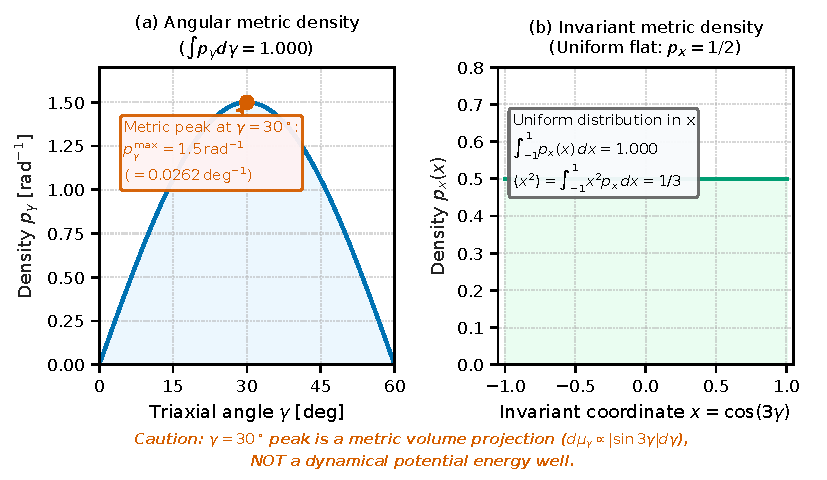
\includegraphics[width=0.85\textwidth]{Img/gamma-measure.pdf}
\caption{平坦角向势下不同坐标表象的概率密度与几何测度示意图。对于固定 $\beta$、自旋 $I=0$、常角向质量且 $\gamma$ 势平坦的受约束模型基态，在变量 $x=\cos 3\gamma \in [-1, 1]$ 下概率分布为平坦常数 $p_x(x)=1/2$，而在形状角 $\gamma \in [0, \pi/3]$ 下由于体积元测度因子 $\sin 3\gamma$ 呈现分布 $p_\gamma(\gamma)=\frac{3}{2}\sin 3\gamma$，并在 $\gamma=30^\circ$ 处取得极值，展示了同一量子态在不同坐标选择下的测度依赖表象。}
\label{fig:gamma-measure}
\end{figure}
}{}
